\documentclass{cmc}

\begin{document}

\pagestyle{fancy}
\lhead{\textit{\textbf{Computational Motor Control, Spring 2019} \\
    Python exercise, Lab 4, NOT GRADED}} \rhead{Student \\ Names}

\section*{Student names: \ldots (please update)}
\textit{Instructions: Update this file (or recreate a similar one,
  e.g.\ in Word) to prepare your answers to the questions. Feel free
  to add text, equations and figures as needed. Hand-written notes,
  e.g.\ for the development of equations, can also be included e.g.\
  as pictures (from your cell phone or from a scanner).  \textbf{This
    lab is not graded. However, the lab exercises are meant as a way
    to familiarise with dynamical systems and to study them using
    Python to prepare you for the final project.} This file does not
  need to be submitted and is provided for your own benefit. The
  graded exercises will have a similar format.}

\textit{The file \fileref{lab\#.py} is provided to run all exercises
  in Python.
  % Each \fileref{exercise\#.py} can be run to run an exercise
  % individually.
  % The list of exercises and their dependencies are shown in
  % Figure~\ref{fig:files}.
  When a file is run, message logs will be printed to indicate
  information such as what is currently being run and and what is left
  to be implemented. All warning messages are only present to guide
  you in the implementation, and can be deleted whenever the
  corresponding code has been implemented correctly.}


\textit{In this exercise, you will explore the different modeling
  techniques that can be used to control a single joint and
  segment. We initially start by exploring a single joint controlled
  by a pair of antagonist spring like muscles and then extend the
  model by adding dampers to it. These only represent the passive
  dynamics observed in a real musculoskeletal system. To make the
  behavior more realistic we then study more complex hill muscle model
  in detail. }

\begin{figure}[ht]
  \centering 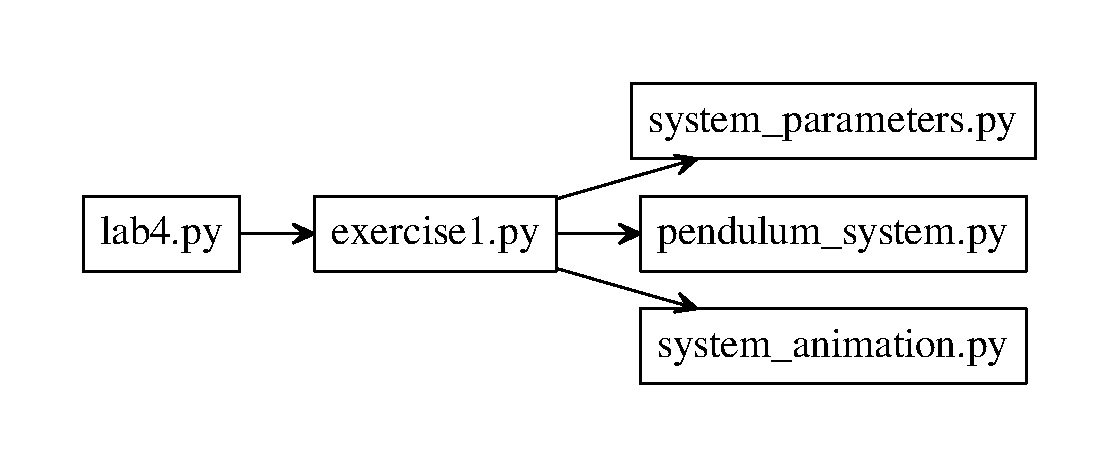
\includegraphics[width=0.5\textwidth]{figures/files}
  \caption{\label{fig:files} Exercise files dependencies. In this lab, you will
    be modifying \fileref{exercise1.py} and \fileref{pendulum\_system.py}}
\end{figure}

\section*{Exercise 1 : Pendulum model with passive elements}
\label{sec:question-1}

Mechanical behavior of muscle tissue can be approximated by simple
passive elements such as springs and dampers. These elements, when
combined properly, allow to study the behavior of muscle under
compressive and tensile loads.

Consider the following equation describing the motion of simple
pendulum with an external torque $T_{ext}$,

\begin{equation}
  \label{eq:pendulum_1}
  I\ddot{\theta} = -mgLsin(\theta) + T_{ext}
\end{equation}

Considering Inertia $I = mL^2$, the equation of the pendulum can be
written as,

\begin{equation}
  \label{eq:pendulum}
  \ddot{\theta} = -g\frac{sin(\theta)}{L} + \frac{T_{ext}}{I}
\end{equation}

Consider the system only for the pendulum range $\theta$ =
$[-\pi/2, \pi/2]$

\subsection*{Explore the pendulum model with two antagonist spring
  elements}

In this question the goal is to add two antagonist springs to the
pendulum model which you are already familiar with from lab 2
exercises. For simplicity we assume the springs directly apply a
torsional force on to the pendulum.  Use equation \ref{eqn:spring} to
develop the spring model.

\textit{\textbf{Note} : The springs can only produce force in
  one-direction like the muscles.  That is, they can only apply a
  pulling force and apply a zero force when compressed.  In terms of
  torsion this translates to, spring S1 can exert only clockwise
  torque and spring S2 can exert only counter-clockwise torque.  You
  need to accommodate for this condition in the equations shown below}

The setup for the pendulum with a pair of antagonist springs is as
shown in figure \ref{fig:pendulum_spring}. Use \fileref{exercise1.py},
\fileref{pendulum\_system.py} and \fileref{system\_parameters.py} files to
complete the exercise.


\begin{figure}[H]
  \centering
  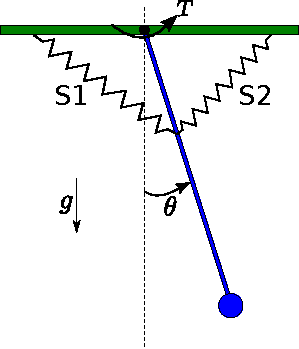
\includegraphics[width=.3\textwidth]{figures/pendulum_spring}
  \caption[pendulum with spring]{Pendulum model with two springs S1
    and S2.\\
    $T$ - Positive torque direction.\\
    $g$ - Gravity.\\
    $\theta$ - Angle made by the pendulum}
  \label{fig:pendulum_spring}
\end{figure}


\begin{equation}
  \label{eqn:spring}
  T_{S} = k*(\theta_{ref} - \theta)
\end{equation}

Where,
\begin{itemize}
\item $T_{S}$ : Torsional Spring force
\item $k$ : Spring Constant
\item $\theta_{ref}$ : Spring reference angle
\item $\theta$ : pendulum angle
\end{itemize}

Substituting the above in \ref{eq:pendulum},

\begin{eqnarray}
  \label{eq:spring}
  \ddot{\theta} = -g\frac{sin(\theta)}{L} + \frac{T_{ext}}{I} + \frac{T_{S}}{I} \\
  \ddot{\theta} = -g\frac{sin(\theta)}{L} + \frac{T_{ext}}{I} + \frac{k*(\theta_{ref} - \theta)}{I} \label{eq:genSpring}
\end{eqnarray}

Use the generalized form of the spring equation described in
\ref{eq:genSpring} to extend it to both the antagonist springs S1 and
S2 with the necessary conditions to make sure springs do not produce
when compressed.



\subsection*{1.a Implement the dynamic equations of the pendulum with
  springs using equations described above in the function
  \fileref{pendulum\_system.py::pendulum\_equation}.  Does the system
  have a stable limit cycle behavior?  Describe and run an experiment
  to support your answer. You can use the function
  \fileref{exercise1.py::pendulum\_perturbation} to perturb the
  pendulum either by changing states or applying an external torque.
  Use the class \fileref{system\_animation.py::SystemAnimation} to
  visualize the pendulum. Example code can be found in
  \fileref{exercise1.py::exercise1}}
\label{subsec:1.a}


\subsection*{1.b Explore the role of spring constant ($k$) and spring
  reference angle ($\theta_{ref}$) in terms of range of motion,
  amplitude and frequency of pendulum. Keep the constants equal, i.e
  $k_1$  = $k_2$ and $\theta_{ref1} = \theta_{ref2}$
  \\ Refer to \fileref{exercise1.py::exercise1} for an example}


\subsection*{1.c Explain the behavior of the model when you have
  asymmetric spring constants ($k$) and spring reference angles
  ($\theta_{ref}$), i.e. $k_1 \neq k_2$ and $\theta_{ref1} \neq \theta_{ref2}$
  Support your responses with relevant plots}


\subsection*{Explore the pendulum model with two antagonist spring and damper elements}
Over time muscles lose energy while doing work. In order to account
for this property, let us now add a damper in parallel to the spring
model. Use equation \ref{eqn:damper} to develop the damper model.

\textit{\textbf{Note} : Like the previous springs, spring-dampers can
  only produce force in one-direction.  That is, together
  spring-damper system can only apply a force in the pulling direction
  and apply a zero force when compressed.  In terms of torsion this
  translates to, spring S1 and damper D1 can each exert only
  clockwise torque and spring S2 and damper D2 can each exert only
  counter-clockwise torque. You need to accommodated for this condition
  in the equations shown below}

Again use \fileref{exercise1.py}, \fileref{pendulum\_system.py} and
\fileref{system\_parameters.py} files to complete the exercise. The
setup for the pendulum model with a pair of antagonist spring and
dampers in parallel is as shown in figure
\ref{fig:pendulum_spring_damper}.


\begin{figure}[H]
  \centering
  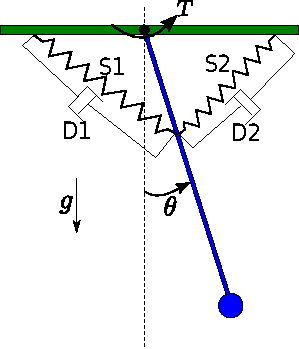
\includegraphics[width=.3\textwidth]{figures/pendulum_spring_damper}
  \caption[pendulum with spring]{Pendulum model with two springs S1
    and S2 and two dampers b1 and b2\\
    $T$ - Positive torque direction.\\
    $g$ - Gravity.\\
    $\theta$ - Angle made by the pendulum}
  \label{fig:pendulum_spring_damper}
\end{figure}



\begin{equation}
  \label{eqn:damper}
  T_{B} = b*(\dot{\theta})
\end{equation}

Where,
\begin{itemize}
\item $T_{B}$ : Torsional Damper force
\item $b$ : Damping Constant
\item $\dot{\theta}$ : pendulum angular velocity
\end{itemize}

The combined spring damper torque is given by,
\begin{equation}
  \label{eq:spring_damper}
  T_{S} - T_{B} = k*(\theta_{ref} - \theta) - b*(\dot{\theta})
\end{equation}

The minus for the damper comes from the fact that damper is acting
against the work done by the spring.

Substituting the above in \ref{eq:pendulum}

\begin{eqnarray}
  \label{eq:spring-damper}
  \ddot{\theta} = -g\frac{sin(\theta)}{L} + \frac{T_{ext}}{I} + \frac{T_{S} - T_{B}}{I} \\
  \ddot{\theta} = -g\frac{sin(\theta)}{L}+ \frac{T_{ext}}{I} + (\frac{k*(\theta_{ref} - \theta) - b*(\dot{\theta})}{I}) \label{eq:genSpringDamper}
\end{eqnarray}

Use the generalized form of the spring equation described in
\ref{eq:genSpringDamper} to extend it to both the antagonist
spring-damper systems (S1-D1) and (S2-D2).


\subsection*{1.d Implement the dynamics equations of the pendulum to
  now include the damping using the equations described above. Modify
  \fileref{pendulum\_system.py::pendulum\_equation}.  How does the
  behavior now change compared to the pendulum without dampers? Briefly explain and support your
  responses with relevant plots}


\subsection*{1.e Can you find a combination of spring constants ($k$),
  damping constants ($b$) and spring reference angles ($\theta_{ref}$)
  that makes the pendulum rest in a stable equilibrium at
  ($\theta = \pi/6$) radians? Describe how you arrive at the necessary
  parameters and support your response with relevant plots.}


\subsection*{1.f What is the missing component between a real muscle
  and the muscle model with passive components that you just explored?
  What behavior's do you lack because of this missing component?}

\end{document}

%%% Local Variables:
%%% mode: latex
%%% TeX-master: t
%%% End: